\documentclass{article}
\usepackage[utf8]{inputenc}
\usepackage{graphicx}
\begin{document}
\section*{A first order differential equation}
Many of the differential equations we come across in neuroscience are
inhomogeneous first order differential equations
\begin{equation}
\tau\frac{df}{dt}=g(t)-f(t)
\end{equation}
where $f(t)$ is some function of $t$ we are interested, $g(t)$ is some
outside \textsl{driving function} and $\tau$ is a constant. In one
example we will examine is the integrate and fire equation:
\begin{equation}
\tau_m\frac{dV}{dt}=E_l-V(t)+g_lI(t)
\end{equation}
where $V(t)$ is the voltage inside a neuron, and the driving function
is made up of two parts $E_l$, the so called reversal potential and
$g_lI(t)$ which represents current coming in to the cell, for example,
through an electrode if the cell being modelled is being experimented
on, or because of signals from other neurons. Another example is the
gating equation which represents the opening and closing of
ino-channels, little gates in the membrane of the cells and a third
example is the equation for synaptic conductance. In each of these
examples the underlying equation is the same, or nearly the same, and
so we will look at it now in the abstract without considering the
application.


These are called first order linear differential equations, first
order because the highest derivative is $df/dt$, there is no
$d^2f/dt^2$ term for example, and linear because there are no
non-linear $f$ terms, no $f^2$ or anything like that. First order
linear differential equations can be solved, or, at least the solution
can be written as an integral. The solution uses an
\textsl{integrating factor}: the trick of simplifying the equation by
multiply across by
\begin{equation}
\lambda=e^{-t/\tau}
\end{equation}
This gives
\begin{equation}
\tau e^{t/\tau}\frac{df}{dt}+e^{t/\tau}f=e^{t/\tau}g(t)
\end{equation}
The clever bit, now, is that the two terms on the right hand side can
be rewritten in product form
\begin{equation}
\tau \frac{d}{dt}\left(e^{t/\tau}f\right)=e^{t/\tau}g(t)
\end{equation}
We integrate both sides
\begin{equation}
\tau e^{t/\tau}f(t)=\int_0^t e^{t'/\tau} g(t')dt'+A
\end{equation}
where $A$ is some integration constant. Setting $t=0$ shows that $A=\tau f(0)$ and, hence, dividing across by the stuff in front of $f(t)$
\begin{equation}
f(t)=e^{-t/\tau}\left[\frac{1}{\tau}\int_0^t e^{t'/\tau} g(t')dt'+f(0)\right]
\end{equation}
Hence, $f(t)$ is written as an integral, if we can do the integral we
have solved the equation.

The easiest case is obviously $g(t)=\bar{g}$ a constant:
\begin{equation}
f(t)= \bar{g} \left[\frac{1}{\tau}e^{-t/\tau}\int_0^t e^{t'/\tau}dt'+f(0)\right]=\bar{g}\left(1-e^{-t/\tau}\right) + f(0)e^{-t/\tau}
\end{equation}
or
\begin{equation}
f(t)=\bar{g}+[f(0)-\bar{g}]e^{-t/\tau}
\end{equation}
It is easy to understand this solution: 
\begin{equation}
\tau\frac{df}{dt}=\bar{g}-f(t)
\end{equation}
has $df/dt=0$ only if $f(t)=\bar{g}$ furthermore if $f(t)>\bar{g}$
then $df/dt<0$ and $f(t)$ decreases towards $\bar{g}$; if
$f(t)>\bar{g}$ $df/dt>0$ then $f(t)$ increases. Since $df/dt$ is zero
for $f(t)=\bar{g}$ we say this is the equilibrium; since the sign of
$df/dt$ means that $f(t)$ always approaches $\bar{g}$ we say this
solution is stable.


We can see in the
solution that $f(t)$ decays exponentially towards $\bar{g}$ and it
does so with a time scale that depends on $\tau$. An example is shown in Fig.~\ref{exp_decay}.

\begin{figure}[tb]
\begin{center}
% GNUPLOT: LaTeX picture with Postscript
\setlength{\unitlength}{0.0500bp}%
\begin{picture}(4320,3024)(0,0)%
  \put(2469,140){\makebox(0,0){\strut{}$t$}}%
  \put(0,0){\includegraphics{exp_decay.eps}}%
  \put(360,1712){\makebox(0,0){\strut{}$f(t)$}}%
  \put(3959,440){\makebox(0,0){\strut{} 20}}%
  \put(3214,440){\makebox(0,0){\strut{} 15}}%
  \put(2470,440){\makebox(0,0){\strut{} 10}}%
  \put(1725,440){\makebox(0,0){\strut{} 5}}%
  \put(980,440){\makebox(0,0){\strut{} 0}}%
  \put(860,2783){\makebox(0,0)[r]{\strut{} 2.5}}%
  \put(860,2247){\makebox(0,0)[r]{\strut{} 2}}%
  \put(860,1712){\makebox(0,0)[r]{\strut{} 1.5}}%
  \put(860,1176){\makebox(0,0)[r]{\strut{} 1}}%
  \put(860,640){\makebox(0,0)[r]{\strut{} 0.5}}%
\end{picture}

\end{center}
\caption{Two examples of $f(t)$ decaying towards $\bar{g}$. Here
  $\bar{g}=1$ and $\tau=10$; in the top curve $f(0)=2.5$ whereas in
  the other $f(0)=0.5$. \label{exp_decay}}
\end{figure}

What happens if $g(t)$ isn't constant; well some of the same logic applies, the sign of $df/dt$ means that the solution is trying to get to $g(t)$ but the difference is now that $g(t)$ might change before it gets there. Actually looking at 
\begin{equation}
f(t)=e^{-t/\tau}\left[\frac{1}{\tau}\int_0^t e^{t'/\tau} g(t')dt'+f(0)\right]
\end{equation}
lets consider the function
\begin{equation}
T(t)=\frac{1}{\tau}e^{-t/\tau}\int_0^t e^{t'/\tau} g(t')dt'
\end{equation}
and do a change of variable $t'=t-s$ so 
\begin{equation}
T(t)=\frac{1}{\tau}\int_0^t e^{-s/\tau} g(t-s)ds
\end{equation}
then the role of the integral is to filter or smooth out $g(t)$ by
averaging it over its past with a exponential window. This is
illustrated in Fig.~\ref{filtering}.

\begin{figure}[tb]
\begin{center}
% GNUPLOT: LaTeX picture with Postscript
\begingroup
  \makeatletter
  \providecommand\color[2][]{%
    \GenericError{(gnuplot) \space\space\space\@spaces}{%
      Package color not loaded in conjunction with
      terminal option `colourtext'%
    }{See the gnuplot documentation for explanation.%
    }{Either use 'blacktext' in gnuplot or load the package
      color.sty in LaTeX.}%
    \renewcommand\color[2][]{}%
  }%
  \providecommand\includegraphics[2][]{%
    \GenericError{(gnuplot) \space\space\space\@spaces}{%
      Package graphicx or graphics not loaded%
    }{See the gnuplot documentation for explanation.%
    }{The gnuplot epslatex terminal needs graphicx.sty or graphics.sty.}%
    \renewcommand\includegraphics[2][]{}%
  }%
  \providecommand\rotatebox[2]{#2}%
  \@ifundefined{ifGPcolor}{%
    \newif\ifGPcolor
    \GPcolorfalse
  }{}%
  \@ifundefined{ifGPblacktext}{%
    \newif\ifGPblacktext
    \GPblacktexttrue
  }{}%
  % define a \g@addto@macro without @ in the name:
  \let\gplgaddtomacro\g@addto@macro
  % define empty templates for all commands taking text:
  \gdef\gplbacktext{}%
  \gdef\gplfronttext{}%
  \makeatother
  \ifGPblacktext
    % no textcolor at all
    \def\colorrgb#1{}%
    \def\colorgray#1{}%
  \else
    % gray or color?
    \ifGPcolor
      \def\colorrgb#1{\color[rgb]{#1}}%
      \def\colorgray#1{\color[gray]{#1}}%
      \expandafter\def\csname LTw\endcsname{\color{white}}%
      \expandafter\def\csname LTb\endcsname{\color{black}}%
      \expandafter\def\csname LTa\endcsname{\color{black}}%
      \expandafter\def\csname LT0\endcsname{\color[rgb]{1,0,0}}%
      \expandafter\def\csname LT1\endcsname{\color[rgb]{0,1,0}}%
      \expandafter\def\csname LT2\endcsname{\color[rgb]{0,0,1}}%
      \expandafter\def\csname LT3\endcsname{\color[rgb]{1,0,1}}%
      \expandafter\def\csname LT4\endcsname{\color[rgb]{0,1,1}}%
      \expandafter\def\csname LT5\endcsname{\color[rgb]{1,1,0}}%
      \expandafter\def\csname LT6\endcsname{\color[rgb]{0,0,0}}%
      \expandafter\def\csname LT7\endcsname{\color[rgb]{1,0.3,0}}%
      \expandafter\def\csname LT8\endcsname{\color[rgb]{0.5,0.5,0.5}}%
    \else
      % gray
      \def\colorrgb#1{\color{black}}%
      \def\colorgray#1{\color[gray]{#1}}%
      \expandafter\def\csname LTw\endcsname{\color{white}}%
      \expandafter\def\csname LTb\endcsname{\color{black}}%
      \expandafter\def\csname LTa\endcsname{\color{black}}%
      \expandafter\def\csname LT0\endcsname{\color{black}}%
      \expandafter\def\csname LT1\endcsname{\color{black}}%
      \expandafter\def\csname LT2\endcsname{\color{black}}%
      \expandafter\def\csname LT3\endcsname{\color{black}}%
      \expandafter\def\csname LT4\endcsname{\color{black}}%
      \expandafter\def\csname LT5\endcsname{\color{black}}%
      \expandafter\def\csname LT6\endcsname{\color{black}}%
      \expandafter\def\csname LT7\endcsname{\color{black}}%
      \expandafter\def\csname LT8\endcsname{\color{black}}%
    \fi
  \fi
  \setlength{\unitlength}{0.0500bp}%
  \begin{picture}(5760.00,4032.00)%
    \gplgaddtomacro\gplbacktext{%
      \csname LTb\endcsname%
      \put(726,704){\makebox(0,0)[r]{\strut{} 0}}%
      \put(726,1470){\makebox(0,0)[r]{\strut{} 0.5}}%
      \put(726,2236){\makebox(0,0)[r]{\strut{} 1}}%
      \put(726,3001){\makebox(0,0)[r]{\strut{} 1.5}}%
      \put(726,3767){\makebox(0,0)[r]{\strut{} 2}}%
      \put(858,484){\makebox(0,0){\strut{} 0}}%
      \put(1421,484){\makebox(0,0){\strut{} 5}}%
      \put(1984,484){\makebox(0,0){\strut{} 10}}%
      \put(2547,484){\makebox(0,0){\strut{} 15}}%
      \put(3111,484){\makebox(0,0){\strut{} 20}}%
      \put(3674,484){\makebox(0,0){\strut{} 25}}%
      \put(4237,484){\makebox(0,0){\strut{} 30}}%
      \put(4800,484){\makebox(0,0){\strut{} 35}}%
      \put(5363,484){\makebox(0,0){\strut{} 40}}%
      \put(3110,154){\makebox(0,0){\strut{}$t$}}%
    }%
    \gplgaddtomacro\gplfronttext{%
      \csname LTb\endcsname%
      \put(4376,3594){\makebox(0,0)[r]{\strut{}$f(t)$}}%
      \put(4376,3374){\makebox(0,0)[r]{\strut{}$g(t)$}}%
    }%
    \gplbacktext
    \put(0,0){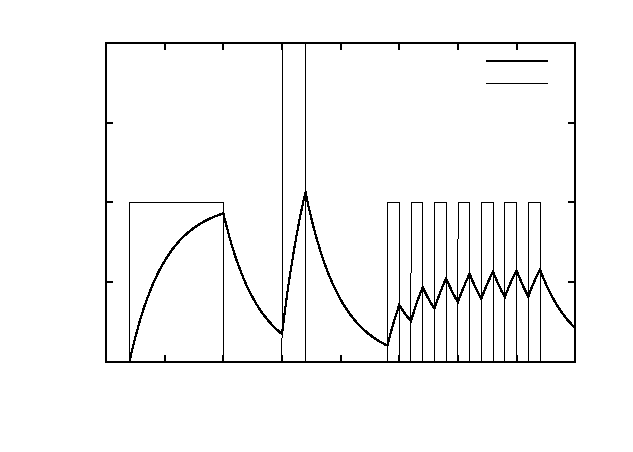
\includegraphics{filtering}}%
    \gplfronttext
  \end{picture}%
\endgroup

\end{center}
\caption{This shows how the response $f(t)$ filters the input $g(t)$;
  the differntial equation has $\tau=3$ and an input $g(t)$ which
  varies as shown above; the coded used to calculate $f(t)$ is
  \texttt{filtered\_input.py}. \label{filtering}}
\end{figure}

Imagine that $g(t)$ varies slowly compared to the time scale $\tau$, so by the time $g(t-s)$ changes much compared to $g(t)$ then $\exp(-s/\tau)$ is more-or-less zero, then
\begin{equation}
T(t)\approx\frac{1}{\tau}g(t)\int_0^t e^{-s/\tau}ds=g(t)\left(1-e^{-t/\tau}\right)
\end{equation}
and substituting back in we get
\begin{equation}
f(t)\approx g(t)+[f(0)-g(t)]e^{-t/\tau}
\end{equation}

\section*{Two first order differential equation}

Differential equations can be coupled; here is an example of a nearly homogeneous pair of coupled equations
\begin{eqnarray}
\tau_f \frac{df}{dt}&=&\bar{f}-f-w\\
\tau_w \frac{dw}{dt}&=&\bar{w}-w
\end{eqnarray}
There are lots of ways to solve this equation; one approach is to
rewrite it as a matrix equation and find the eigenvectors, another is
to convert it into a second order equation and solve that; the first
way is more general but the second is quicker. Let's start by making
the equation homogeneous and going from there, so let
\begin{eqnarray}
f'&=&f-\bar{f}-\bar{w}\\
w'&=&w-\bar{w}
\end{eqnarray}
giving
\begin{eqnarray}
\tau_f \frac{df'}{dt}&=&-f'-w'\\
\tau_w \frac{dw'}{dt}&=&-w'
\end{eqnarray}
Actually having the prime on $f$ and $w$ gets annoying so we'll drop the prime for convenience.
\begin{eqnarray}
\tau_f \frac{df}{dt}&=&-f-w\\
\tau_w \frac{dw}{dt}&=&-w
\end{eqnarray}

Now, differenciate the first equation to get
\begin{equation}
\tau_f \frac{d^2f}{dt^2}=-\frac{df}{dt}-\frac{dw}{dt}
\end{equation}
Since 
\begin{equation}
\frac{dw}{dt}=-\frac{1}{\tau_w}w
\end{equation}
we can substitute back in for $w$:
\begin{equation}
\tau_f \frac{d^2f}{dt^2}=-\frac{df}{dt}+\frac{1}{\tau_w}w
\end{equation}
From the original $df/dt$ equation we have
\begin{equation}
w=-f-\tau_f \frac{df}{dt}
\end{equation}
and using this to get rid of the $w$ we have
\begin{equation}
\tau_f \frac{d^2f}{dt^2}=-\frac{df}{dt}-\frac{1}{\tau_w}f-\frac{\tau_f}{\tau_w}\frac{df}{dt}
\end{equation}
Finally, multiplying across by $\tau_w$ and fiddling around a bit we have
\begin{equation}
\tau_w\tau_f \frac{d^2f}{dt^2}+(\tau_w+\tau_f)\frac{df}{dt}+f=0
\end{equation}

This second order equation is solved by ansatz, that is by guessing; we guess
\begin{equation}
f(t)=e^{rt}
\end{equation}
and substitute back in
\begin{equation}
\tau_w\tau_f r^2+(\tau_w+\tau_f)r+1=0
\end{equation}
which has two solutions $r=-1/\tau_f$ and $r=-1/\tau_w$ so
\begin{equation}
f(t)=Ae^{-t/\tau_f}+Be^{-t/\tau_w}
\end{equation}
and substituting back into 
\begin{equation}
\tau_f \frac{df'}{dt}=-f'-w'
\end{equation}
give an equation for $w'$.

Another approach to this pair of equations which we won't explore here
is to write them as a matrix equation:
\begin{equation}
\frac{d}{dt}\left(\begin{array}{c}f'\\w'\end{array}\right)
=\left(\begin{array}{cc}-1/\tau_f&-1/\tau_f\\0&-1/\tau_w\end{array}\right)
\left(\begin{array}{c}f'\\w'\end{array}\right)
\end{equation}

As important as seeing how to solve these differential equation is
understanding the phase dynamics; recall how in case above with just
one differential equation we could see that the equation had a stable
equilibrium, well we can do the same thing here. First consider the equation
\begin{equation}
\tau_w \frac{dw}{dt}=-w
\end{equation}
If $w=0$ this means that $dw/dt=0$; this is called a nullcline and, in
$f-w$ space it is a line not a point. The system isn't in equilibrium
along the nullcline because $df/dt$ isn't zero but it is stable in the
sense that if we are above $w=0$ then $dw/dt<0$ and if it is below
$dw/dt>0$ and so, as before, the system will approach the
nullcline. In fact there is also a $df/dt$ nullcline given by $f=-w$;
this is a diagonal line in $f-w$ space; it is also stable, if $f>-w$,
that is if we are to the right of the nullcline, then $df/dt<0$ and we
move to the left, and the converse for $f<-w$. Hence, we always move
towards the nullclines; furthermore, the two lines cross at $f=w=0$
and this is a stable equilibrium point.


\begin{figure}[tb]
\begin{center}
% GNUPLOT: LaTeX picture with Postscript
\begingroup
  \makeatletter
  \providecommand\color[2][]{%
    \GenericError{(gnuplot) \space\space\space\@spaces}{%
      Package color not loaded in conjunction with
      terminal option `colourtext'%
    }{See the gnuplot documentation for explanation.%
    }{Either use 'blacktext' in gnuplot or load the package
      color.sty in LaTeX.}%
    \renewcommand\color[2][]{}%
  }%
  \providecommand\includegraphics[2][]{%
    \GenericError{(gnuplot) \space\space\space\@spaces}{%
      Package graphicx or graphics not loaded%
    }{See the gnuplot documentation for explanation.%
    }{The gnuplot epslatex terminal needs graphicx.sty or graphics.sty.}%
    \renewcommand\includegraphics[2][]{}%
  }%
  \providecommand\rotatebox[2]{#2}%
  \@ifundefined{ifGPcolor}{%
    \newif\ifGPcolor
    \GPcolorfalse
  }{}%
  \@ifundefined{ifGPblacktext}{%
    \newif\ifGPblacktext
    \GPblacktexttrue
  }{}%
  % define a \g@addto@macro without @ in the name:
  \let\gplgaddtomacro\g@addto@macro
  % define empty templates for all commands taking text:
  \gdef\gplbacktext{}%
  \gdef\gplfronttext{}%
  \makeatother
  \ifGPblacktext
    % no textcolor at all
    \def\colorrgb#1{}%
    \def\colorgray#1{}%
  \else
    % gray or color?
    \ifGPcolor
      \def\colorrgb#1{\color[rgb]{#1}}%
      \def\colorgray#1{\color[gray]{#1}}%
      \expandafter\def\csname LTw\endcsname{\color{white}}%
      \expandafter\def\csname LTb\endcsname{\color{black}}%
      \expandafter\def\csname LTa\endcsname{\color{black}}%
      \expandafter\def\csname LT0\endcsname{\color[rgb]{1,0,0}}%
      \expandafter\def\csname LT1\endcsname{\color[rgb]{0,1,0}}%
      \expandafter\def\csname LT2\endcsname{\color[rgb]{0,0,1}}%
      \expandafter\def\csname LT3\endcsname{\color[rgb]{1,0,1}}%
      \expandafter\def\csname LT4\endcsname{\color[rgb]{0,1,1}}%
      \expandafter\def\csname LT5\endcsname{\color[rgb]{1,1,0}}%
      \expandafter\def\csname LT6\endcsname{\color[rgb]{0,0,0}}%
      \expandafter\def\csname LT7\endcsname{\color[rgb]{1,0.3,0}}%
      \expandafter\def\csname LT8\endcsname{\color[rgb]{0.5,0.5,0.5}}%
    \else
      % gray
      \def\colorrgb#1{\color{black}}%
      \def\colorgray#1{\color[gray]{#1}}%
      \expandafter\def\csname LTw\endcsname{\color{white}}%
      \expandafter\def\csname LTb\endcsname{\color{black}}%
      \expandafter\def\csname LTa\endcsname{\color{black}}%
      \expandafter\def\csname LT0\endcsname{\color{black}}%
      \expandafter\def\csname LT1\endcsname{\color{black}}%
      \expandafter\def\csname LT2\endcsname{\color{black}}%
      \expandafter\def\csname LT3\endcsname{\color{black}}%
      \expandafter\def\csname LT4\endcsname{\color{black}}%
      \expandafter\def\csname LT5\endcsname{\color{black}}%
      \expandafter\def\csname LT6\endcsname{\color{black}}%
      \expandafter\def\csname LT7\endcsname{\color{black}}%
      \expandafter\def\csname LT8\endcsname{\color{black}}%
    \fi
  \fi
  \setlength{\unitlength}{0.0500bp}%
  \begin{picture}(5760.00,4032.00)%
    \gplgaddtomacro\gplbacktext{%
      \csname LTb\endcsname%
      \put(2715,264){\makebox(0,0)[r]{\strut{}-10}}%
      \put(2715,614){\makebox(0,0)[r]{\strut{}-8}}%
      \put(2715,965){\makebox(0,0)[r]{\strut{}-6}}%
      \put(2715,1315){\makebox(0,0)[r]{\strut{}-4}}%
      \put(2715,1665){\makebox(0,0)[r]{\strut{}-2}}%
      \put(2715,2016){\makebox(0,0)[r]{\strut{} 0}}%
      \put(2715,2366){\makebox(0,0)[r]{\strut{} 2}}%
      \put(2715,2716){\makebox(0,0)[r]{\strut{} 4}}%
      \put(2715,3066){\makebox(0,0)[r]{\strut{} 6}}%
      \put(2715,3417){\makebox(0,0)[r]{\strut{} 8}}%
      \put(2715,3767){\makebox(0,0)[r]{\strut{} 10}}%
      \put(330,1733){\makebox(0,0){\strut{}-10}}%
      \put(833,1733){\makebox(0,0){\strut{}-8}}%
      \put(1337,1733){\makebox(0,0){\strut{}-6}}%
      \put(1840,1733){\makebox(0,0){\strut{}-4}}%
      \put(2343,1733){\makebox(0,0){\strut{}-2}}%
      \put(2847,1733){\makebox(0,0){\strut{} 0}}%
      \put(3350,1733){\makebox(0,0){\strut{} 2}}%
      \put(3853,1733){\makebox(0,0){\strut{} 4}}%
      \put(4356,1733){\makebox(0,0){\strut{} 6}}%
      \put(4860,1733){\makebox(0,0){\strut{} 8}}%
      \put(5363,1733){\makebox(0,0){\strut{} 10}}%
    }%
    \gplgaddtomacro\gplfronttext{%
    }%
    \gplbacktext
    \put(0,0){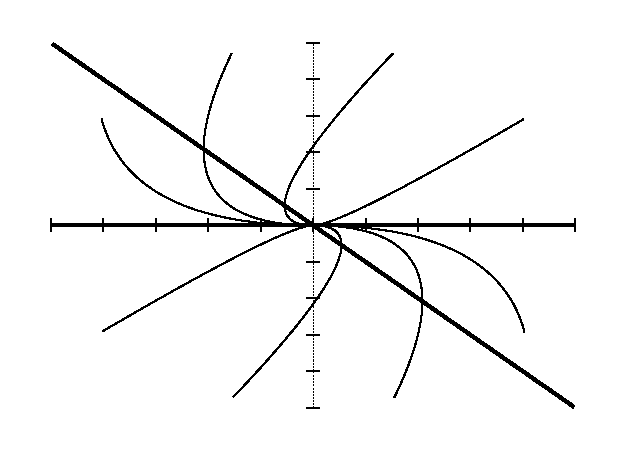
\includegraphics{two_d}}%
    \gplfronttext
  \end{picture}%
\endgroup

\end{center}
\caption{This shows some of the trajectories in $f-w$ space; the
  horizontal axis is $f$, the vertical is $w$. The nullclines are the
  two curves in bold. All the trajectories approach the equilibrium
  point, as they cross the $f=-w$ nullcline their tangent is vertical
  because on this line $df/dt=0$; $\tau_f=2$ and $\tau_w=1$; the programme is
  \texttt{two\_d.py}. \label{two_d}}
\end{figure}


\end{document}


































\end{document}
